\chapter{Theory exercises}

\section{LO DIS}
\label{app:LO}
We are recomputing the LO DIS cross section depicted in \cref{fig:LODIS} in full generality.
\begin{figure}
    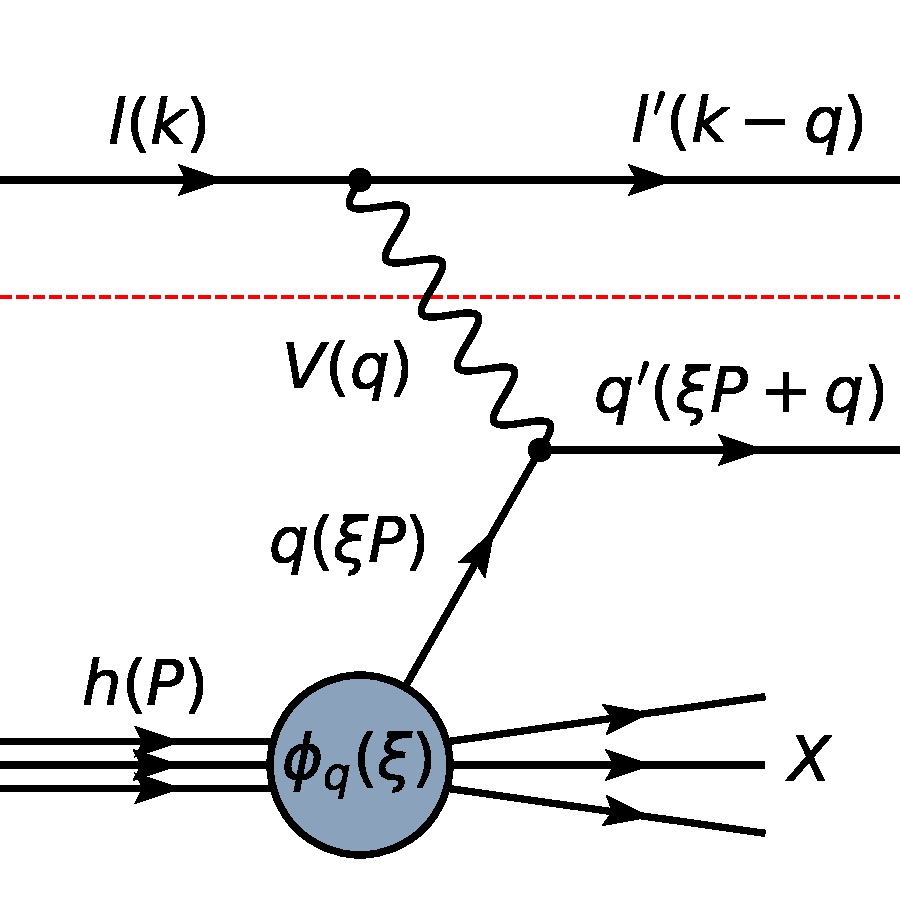
\includegraphics[width=.5\textwidth]{figures/LODIS.pdf}
    \caption{LO DIS Feynman diagram: $l + h \to l' + X$}
    \label{fig:LODIS}
\end{figure}
As we say in \cref{sec:xs} we can decompose the full cross section into a leptonic tensor $L_{\mu\nu}$ and a hadronic tensor $W_{\mu\nu}$ where the red line indicates the split.
In the collinear framework it is sufficient to compute the partonic (sub-)diagram $l + q \to l' + q' + X$.
The parton-in-hadron amplitude $\phi_q$ combines upon taking the modulus square of the whole amplitude together with the inclusiveness $X$ into the PDF $f_q(\xi)$.
This leaves us essentially with twice \cref{fig:LO}, once for the leptonic side and once for the quark side.
Since the fermion lines are distinct we can compute them one at a time and if we keep them general enough we only need to do it once.
Note that we first compute the lepton tensor, i.e.\ we keep the vector boson coupling Lorentz-index open and different in the amplitude and its complex conjugate.

In the first step we only deal with the Dirac structures.
We need the following Feynman rules
\begin{itemize}
    \item outgoing fermion $\bar u(k')$
    \item vector boson-fermion interaction $\Gamma_\mu$, which we make concrete below
    \item incoming fermion $u(k)$
\end{itemize}
and we assume massless fermions in this exercise.
Thus we have
\begin{equation}
    \text{\cref{fig:LO}} = \mathcal A_\mu = \bar u(k')\Gamma_\mu u(k)
\end{equation}
where we have suppressed any additional dependency and we need to compute
\begin{equation}
    T_{\mu\nu} = A_\mu A_\nu^* \,.
\end{equation}

We recall some relevant Dirac traces:
\begin{align}
    \tr(\mathbbm 1) &= 4 \\
    \tr(\gamma_\mu) &= 0 \\
    \tr(\gamma_\mu\gamma_\nu) &= 4g_{\mu\nu} \\
    \tr(\gamma_\mu\gamma_\nu\gamma_\rho) &= 0 \\
    \tr(\gamma_\mu\gamma_\nu\gamma_\rho\gamma_\sigma) &= 4(g_{\mu\nu}g_{\rho\sigma} - g_{\mu\rho}g_{\nu\sigma} + g_{\mu\sigma}g_{\nu\rho})
\end{align}
We also need the simple anti-commutating $\gamma_5$, with properties
\begin{equation}
    \gamma_5 = \frac i {4!}\varepsilon^{\mu\nu\rho\sigma}\gamma_\mu\gamma_\nu\gamma_\rho\gamma_\sigma, \quad \gamma_5\gamma_\mu = - \gamma_\mu\gamma_5, \quad \gamma_5\gamma_5 = \mathbbm 1
\end{equation}
and the corresponding Dirac traces
\begin{equation}
    \tr(\gamma_5) = \tr(\gamma_\mu\gamma_5) = \tr(\gamma_\mu\gamma_\nu\gamma_5) = \tr(\gamma_\mu\gamma_\nu\gamma_\rho\gamma_5) = 0
\end{equation}
and
\begin{equation}
    \tr(\gamma_\mu\gamma_\nu\gamma_\rho\gamma_\sigma\gamma_5) = 4i\varepsilon_{\mu\nu\rho\sigma}\,.
\end{equation}

We start by assuming $\Gamma_\mu = \gamma_\mu$ and averaging over fermion spins $s$ upon which the spinors collapse to just, e.g., $\slashed{k}$.
\begin{exercisebox}{Step 1}
    Proof
    \begin{align}
        T^1_{\mu\nu} &= \frac 1 2 \sum_{s} \bar u^{(s)}(k')\gamma_\mu u^{(s)}(k) \left(\bar u^{(s)}(k')\gamma_\nu u^{(s)}(k)\right)^*\\
         &= 2\left(k_\mu k'_\nu + k_\nu k'_\mu - k \cdot k' g_{\mu\nu}\right)
    \end{align}
\end{exercisebox}
\noindent $T^1_{\mu\nu}$ becomes the spin-averaged leptonic tensor $L_{\mu\nu}$ for photons when choosing the lepton kinematics.

Next, we give up on averaging and instead consider fermions with definite helicities\footnote{Helicity is more convenient than spin in this context}.
For spinors with a given helicity $\lambda = \pm 1$ we find
\begin{equation}
    u(k,\lambda) \bar u(k,\lambda) = \frac 1 2 \slashed k (1 - \lambda \gamma_5) \,.
\end{equation}
\begin{exercisebox}{Step 2}
    Proof
    \begin{align}
        T^2_{\mu\nu} &= \bar u(k',\lambda)\gamma_\mu u(k,\lambda) \left(\bar u(k',\lambda)\gamma_\nu u(k,\lambda)\right)^*\\
         &= T^1_{\mu\nu} + 2 i \lambda \varepsilon_{\mu\nu\rho\sigma} k^\rho k'^\sigma
    \end{align}
\end{exercisebox}
\noindent $T^2_{\mu\nu}$ becomes the leptonic tensor $L_{\mu\nu}^\gamma$ for photons when choosing the lepton kinematics.

Next, we want to use a more realistic boson-fermion coupling $\Gamma_\mu$, since eventually we need to consider the interference between a purely vectorial boson, such as the photon, and the $Z$ boson, which has a mixture between a vectorial coupling and an axial vectorial coupling,
\begin{equation}
    \Gamma^{ph}_\mu = g_V^{\gamma f}\gamma_\mu\,, \qquad \Gamma^Z_\mu = \gamma_\mu(g_V^{Z f} - g_A^{Z f} \gamma_5)
\end{equation}
where $g_V^{\gamma f}$ is the coupling strength between the photon and the fermion $f$ and $g_V^{Z f}$ and $g_A^{Z f}$ are the vectorial and axial-vectorial coupling strength between the Z boson and the fermion $f$.
By convention we exclude an explicit factor of the elementary electric charge from the definition of $g_{V,A}^{B f}$.
$T^2_{\mu\nu}$ obtains a trivial factor of $(g_V^{\gamma f})^2$ when using $\Gamma^{ph}_\mu$.
\begin{exercisebox}{Step 3}
    Proof
    \begin{align}
        T^3_{\mu\nu} &= \bar u(k',\lambda)\Gamma^Z_\mu u(k,\lambda) \left(\bar u(k',\lambda)\Gamma^{ph}_\nu u(k,\lambda)\right)^*\\
         &= g_V^{\gamma f}(g_V^{Z f} - \lambda g_A^{Z f})T^2_{\mu\nu}
    \end{align}
\end{exercisebox}
\noindent $T^3_{\mu\nu}$ becomes the leptonic tensor $L_{\mu\nu}^{\gamma Z}$ for the photon-Z interference when choosing the lepton kinematics and couplings.

Finally, we need the pure Z boson contributions.
\begin{exercisebox}{Step 4}
    Proof
    \begin{align}
        T^4_{\mu\nu} &= \bar u(k',\lambda)\Gamma^Z_\mu u(k,\lambda) \left(\bar u(k',\lambda)\Gamma^{Z}_\nu u(k,\lambda)\right)^*\\
         &= (g_V^{Z f} - \lambda g_A^{Z f})^2 T^2_{\mu\nu}
    \end{align}
\end{exercisebox}
\noindent $T^4_{\mu\nu}$ becomes the leptonic tensor $L_{\mu\nu}^{Z}$ for the Z bosons when choosing the lepton kinematics and couplings.

The leptonic tensor $L_{\mu\nu}^{W}$ for the W bosons follows from the Z boson case by choosing appropriate couplings $g_{V,A}^{W f}$.

The lepton kinematics are obtained by choosing the incoming momentum $k$ and the the outgoing momentum $k' = k - q$, \cref{fig:LODIS}.
\begin{exercisebox}{Step 5: Ward identity}
    Proof
    \begin{equation}
        L^j_{\mu\nu} q^\mu = 0 = L^j_{\mu\nu} q^\nu \quad j \in\{\gamma, \gamma Z, Z, W\}
    \end{equation}
\end{exercisebox}

\begin{exercisebox}{Step 6}
    Proof
    \begin{equation}
        L^\gamma_{\mu\nu} g^{\mu\nu} = -2 Q^2
    \end{equation}
\end{exercisebox}

We now turn our attention to the hadronic side, which is essentially identical except the fermion is now the quark and we have to choose different incoming and outgoing momenta.
We define $p = \xi P$ and $T^2_{\mu\nu}$ becomes the photon-quark tensor $\hat W^{\gamma q}_{\mu\nu}$ by choosing the incoming momentum $p$ and the outgoing momentum $p'=p+q$, \cref{fig:LODIS}.
\begin{exercisebox}{Step 7}
    Proof
    \begin{equation}
        L^\gamma_{\mu\nu} P^{\mu} P^{\nu} = \frac{Q^4}{x^2 y^2}(1-y)
    \end{equation}
\end{exercisebox}
\begin{exercisebox}{Step 8}
    Proof
    \begin{equation}
        L^\gamma_{\mu\nu} \hat W^{\mu\nu}_{\gamma q} = 2\frac{Q^4}{z^2 y^2}\left(2-2y + y^2\right)
    \end{equation}
    if we average over helicities.
\end{exercisebox}


\section{RSL}
\label{app:RSL}

\begin{exercisebox}{RSL representation}
    Proof
    \begin{equation}
        C(z) = \left(\frac{\ln(1-z)}{1-z}\right)_+ \,\leftrightarrow\, C^R(z) = 0, C^S(z) = \frac{\ln(1-z)}{1-z}, C^L(x) = \frac{\ln(1-x)^2}{2}
    \end{equation}
\end{exercisebox}

\begin{exercisebox}{Product of functions 1}
    Give the RSL representation of the product a regular function $r(z)$ and a +-distribution $\qty(p(z))_+$, $C(z) = r(z)\qty(p(z))_+$
\end{exercisebox}

\begin{exercisebox}{Product of functions 2}
    Proof
    \begin{equation}
        \left[r(z)p(z)\right]_+ = r(z) \left[p(z)\right]_+ - \delta(1-z) \int\limits_0^1 dy~ r(y) \left[p(y)\right]_+
    \end{equation}
    where again $r(z)$ is a regular function and $\qty(p(z))_+$ is a +-distribution.
\end{exercisebox}

\section{Resummation}

\begin{exercisebox}[label={box:LOalphas}]{LO $\alpha_s$ evolution}
    Proof \cref{eq:LOalphas} can be written as
    \begin{equation}
        \alpha_s(\mu_R^2) = \frac 1 {\beta_0 \ln(\mu_R^2/\LQCD^2)}
    \end{equation}
    and given an explicit expression for $\LQCD$.
\end{exercisebox}
